\section{Castalia Application Layer}\label{castaliaapplayer}

We have created an application for the Castalia Application Layer. This application is agent and manager-initiated, that is, the agent takes the initiative to send readings to the manager or the manager may request measurements to an agent. The agent is the first and the only one to send an \textit{Association request} to start sending measurements. To stop a transmission in agent-initiated mode, agents can send an \textit{Association Release} message when there is no more measurements to be sent. In the manager-initiated mode a \textit{Stop Request} message is send to an agent requesting the stop measurement data transmission.

The proposed application has five agent types: pulse oximeter, glucose meter, thermometer, blood pressure monitor and a basic ECG. The pulse oximeter transmits the pulse rate in beats per second and the percentage of arterial hemoglobin oxygen saturation (SpO$_2$). The glucose meter sends the glucose level, that is, the concentration of glucose in the blood in milligrams per deciliter (mg\//dL). The thermometer measures temperature in Celsius (\textdegree C). The blood pressure sends a data compound of systolic, diastolic and the mean arterial pressure in millimeters of mercury (mmHg). The basic ECG sends eighty samples of the heart's electric potential in millivolt (mV) per packet. Each mV sample has to be converted to scaled non-negatives values before sent. 
%The lower and upper absolute values and the lower and upper scaled values are transmitted in the configuration phase. 
All these agents samples are randomly produced, except the basic ECG that transmits real values obtained from the data base \cite{b2}.

The X73-PHD standard defines \textbf{confirmed} and  \textbf{unconfirmed events}. The confirmed events expect a reception acknowledgment from the manager and the unconfirmed events do not. Control messages, like \textit{Association request} and \textit{Association release}, are always sent in confirmed mode, but measurements can be configured to use confirmed or unconfirmed mode.
The standard also defines three modes of manager-initiated measurement data transmission: \textbf{Single Response}, \textbf{Time Period} and \textbf{No Time Limit Mode}. The Single Response Mode allows the manager to explicitly request a single data from the agent and receive it in the response message.  The Time Period Mode is used by the manager to enable an agent to send any data it collects for the duration of the requested time period. The No Time Limit Mode shall be used to order an agent to send event reports continually until a \textit{Stop Request} message is received or the association between the agent and the manager is terminated.
%The implemented parameter to set the desired mode is \textit{SN.node\[node number\].Application.confirmed\_event} which require a Boolean value.

In our application, the user can set some simulation's parameters like: the medical device type, thermometer, pulse oximeter, blood pressure and etc, the transmission rate in measurements per seconds, the events types confirmed/unconfirmed and the manager-initiated mode data transmission. If no manager-initiated mode is set, the application uses Agent-initiated mode.

\subsection{Unconfirmed measurement event}\label{sec:UnconfirmedMeasurementEvent}

Figure~\ref{fig:unconfirmedMode} shows a sequence diagram of the messaging process corresponding to an ordinary operation of an agent with standard configuration and with unconfirmed measurement events. The agent intends to associate with the manager for the first time, and sends an \textit{Association request}. When the manager receives the \textit{Association request}, it checks if the agent was previously associated. If it is the agent's first association, the manager sends a \textit{Get attributes} message along with the \textit{Association response}. So, the agent sends its configuration and starts to send the measurements to the manager. When there are no more readings to transmit, the agent sends an \textit{Association release} and the manager responds with an \textit{Association release response}.

\begin{figure}[htbp]
\centerline{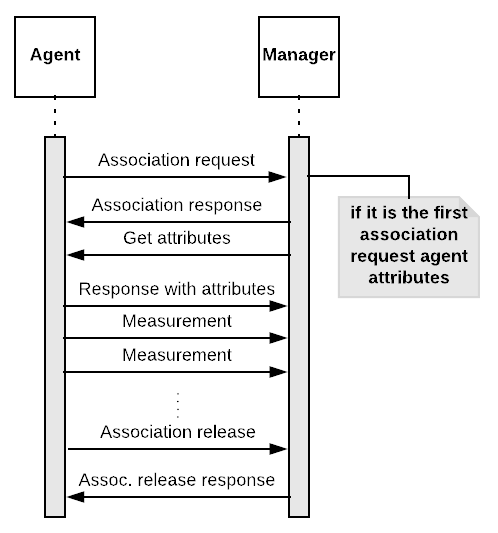
\includegraphics[scale=0.35]{figures/unconfirmed.png}}
\caption{Sequence diagram of unconfirmed operation mode of an 11073 PHD application.}
\label{fig:unconfirmedMode}
\end{figure}

\subsection{Confirmed measurement event}

Figure~\ref{fig:confirmedMode} depicts a sequence diagram of the messaging procedure corresponding to an operation of an agent with standard configuration and with confirmed measurements events. The initial procedure is the same as explained in Section \ref{sec:UnconfirmedMeasurementEvent}, the difference is that the manager sends an acknowledgment for every measurement received. After sending a measurement data, the agent must wait three seconds for an ACK. If an ACK is not received in this period, the agent sends an \textit{Association abort} to the manager, and transits to the unassociated state. If the agent still has readings to send, a new association must be made.

\begin{figure}[htbp]
\centerline{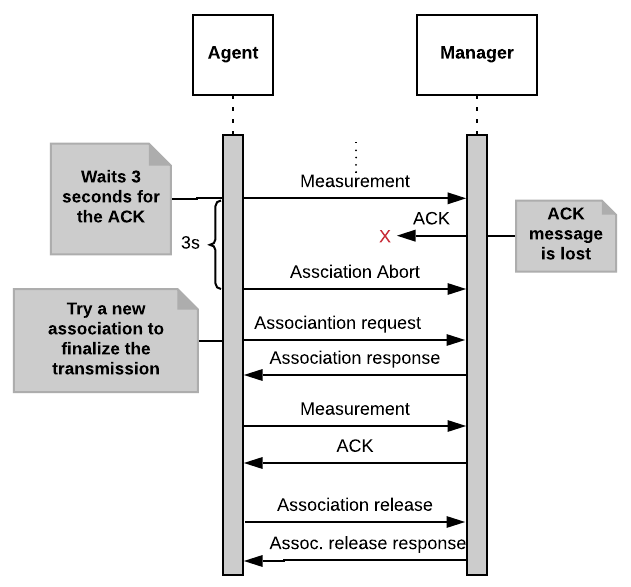
\includegraphics[width=\linewidth]{figures/confirmedModeWithAckLoss.png}}
\caption{Sequence diagram of confirmed operation mode of an 11073 PHD application.}
\label{fig:confirmedMode}
\end{figure}

\subsection{Proposed modification in confirmed measurement events}

The X73-PHD standard assumes that there will be a reliable transport layer on real devices. In the Castalia simulator, as in usual wireless sensor networks, a transport layer could not be used. So we propose a stop-and-wait system as a sub-application-layer to retransmit agent packets whose ACK have not been received.
%To avoid many associations right after a non-received ACK we implemented a stop-and-wait retransmission system in the application layer. 
It reduces the unnecessary exchange of several control packets made in association procedures. Rather than making a new association when an ACK is lost, we just retransmit the packet $n$ times or until an ACK is received.
%The user can define whether to retransmit and how many retransmission attempts wish.
The user may define a number $n$ of retransmissions, and the agent will retransmit that message up to $n$ times until a corresponding ACK is received. If the manager receives a duplicated message, it will retransmit immediately another ACK to the agent. We call it \textbf{Retransmission Mode}.

In Section \ref{results}, we evaluate this solution's efficiency in reducing control packets exchange in a WBAN scenario. Note that this is a new proposal, not present in the X73-PHD standard. In Figure~\ref{fig:retransmissionMode}, is shown a sequence diagram for a data measurement transmission using retransmission mode. In this figure two case are addressed: An ACK for a data measurement is not received and a data measurement is lost.
%The parameters implemented for retransmission are \textit{SN.node[nodeNumber].Application.retransmissionPacket} which require a boolean value and \textit{SN.node[nodeNumber].Application.maxNumOfRetransmition} that accepts an integer number.

\begin{figure}[htbp]
\centerline{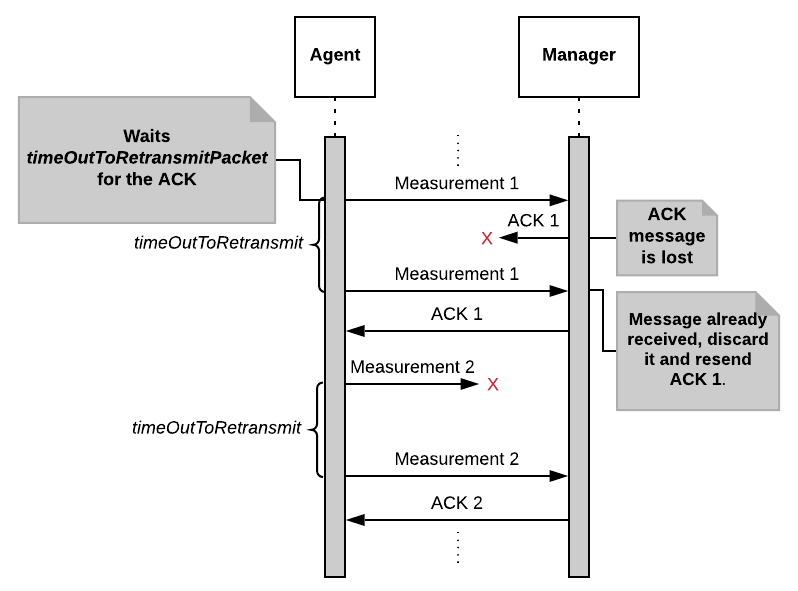
\includegraphics[width=\linewidth]{figures/retransmissionModeWithAckLoss.png}}
\caption{Sequence diagram of retransmission operation mode of an 11073 PHD application.}
\label{fig:retransmissionMode}
\end{figure}

\subsection{Manager-initiated modes}

Figure~\ref{fig:managerinitiated} depicts a sequence diagram of the messaging procedure corresponding to an operation of an agent using manager-initiated events. The initial procedure is the same as explained in above sections. The difference is the \textit{Data Request} control packet. This packet can request measurement data to agents in three ways: Single, Time Period and No Time Period mode. The time has to be defined in Time Period mode.

\begin{figure}[htbp]
\centerline{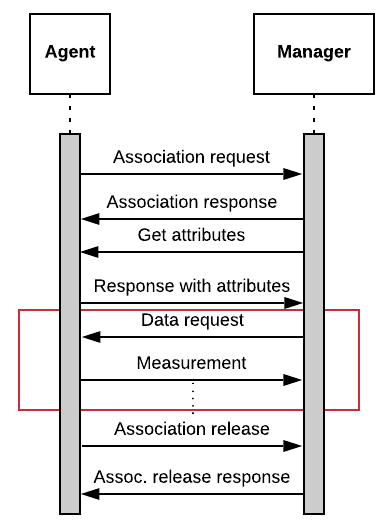
\includegraphics[scale=0.35]{figures/Manager-initiatedmode.png}}
\caption{Sequence diagram of manager-initiated operation mode of an 11073 PHD application}
\label{fig:managerinitiated}
\end{figure}